\section{Format specifications content}

So far the focus has been mainly on the definition of the IACT DL3 formats.  A "general" section defines common things like details about time scales or coordinate systems. Some work on the definition of higher-level formats for spectra and lightcurves is on going. HEALPIX  (Hierarchical Equal Area isoLatitude Pixelization of a sphere) projection for images and  description of data cubes are also considered.

Next sections will describe the effort toward the event list format definition as well as an example for spectra.

\subsection{IACT DL3}

DL3 format should describe all data released to the end users for analysis with science tools as , EVENT, IRF and TECH (technical data not directly attached to the object observed). Figure~\ref{fig:iact-dl3} illustrates some of the DL3 data content. Prototyping by existing IACTs (H.E.S.S., MAGIC, VERITAS and science tools (Gammapy, Ctools) is a major activity. 

\begin{figure}[tb]
  \centerline{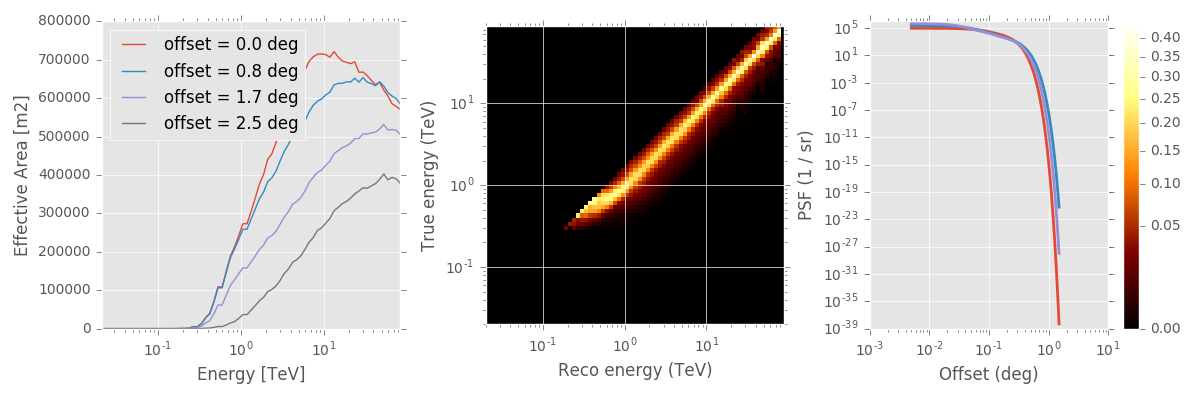
\includegraphics[width=\textwidth]{figures/iact-dl3}}
  \caption{Low-level example: IACT DL3}
  \label{fig:iact-dl3}
\end{figure}

Many points are still under discussion/consideration:

\begin{itemize}
\item{}Observations modes, time intervals
\item{}How to link EVENT and IRF
\item{}Pointing and live time information
\item{}IRF axis and validity ranges
\item{}FoV coordinates
\end{itemize}

\subsection{Likelihood SED and light curves}

A format is developed to store spectral analysis results for exchange and publication, not only "flux points" and "upper limits", but also the full likelihood profiles (see examples in Figure~\ref{fig:dl4-examples}).

\begin{figure}[tb]
\centerline{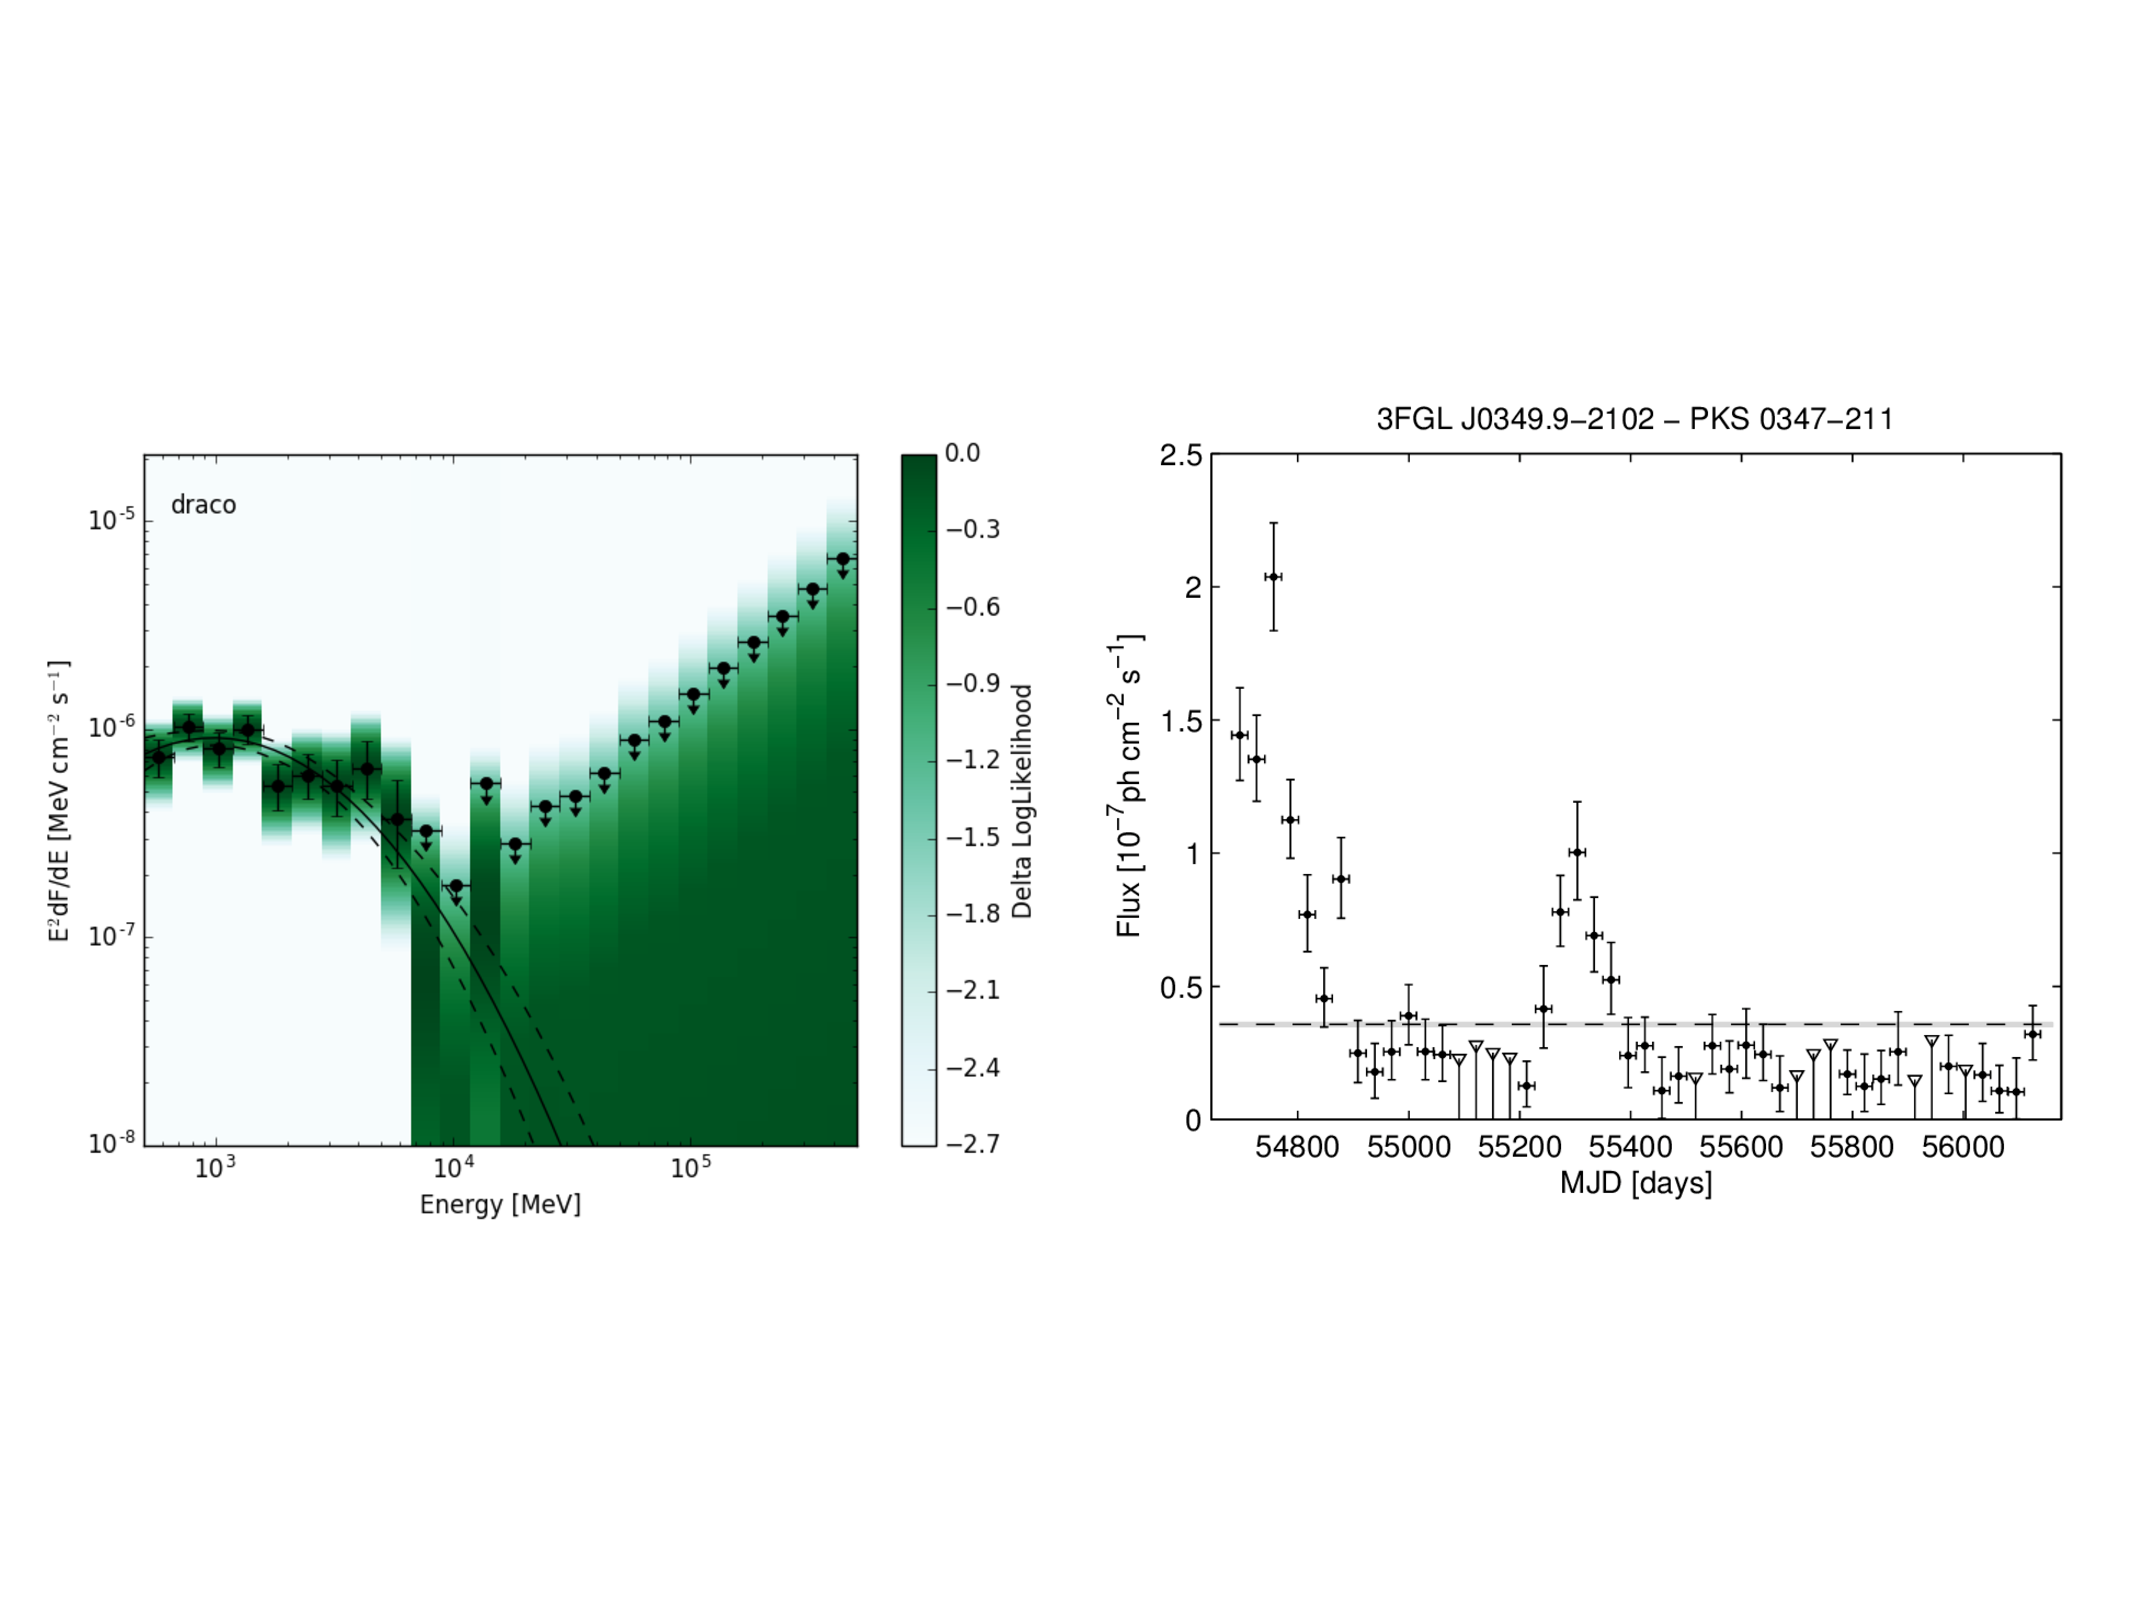
\includegraphics[width=\textwidth]{figures/dl4-examples}}
\caption{
Gamma-ray "data level 4" examples. \emph{Left:} spectral energy distribution (SED) likelihood profiles (green), with flux points and upper limits as well
as a best-model fit overplotted. \emph{Right:} Lightcurve of 3FGL~J0349.9-2102 from the third Fermi-LAT catalog.
}
\label{fig:dl4-examples}
\end{figure}

It was first developed in Fermipy\footnote{\url{https://github.com/fermipy/fermipy}} and used for Fermi-LAT (ref). It is now being adopted by ground-based high energy astronomy. Likelihood profiles are important information when those data are to be used in global spectral energy distribution (SED) of a source. 

Description of light curves is another topic open for discussion. 
